\chapter{Evoluindo uma plataforma de rede social}
\label{evol-rede-social}
%
\section{Noosfero}
\label{noosfero}

O Noosfero \footnote{Disponível em: \url{http://www.noosfero.org}} é uma plataforma de criação de redes sociais livre desenvolvida em 2007 pela Cooperativa de Tecnologias Livres - Colivre \footnote{\url{http://www.colivre.coop.br}}, sob a licença AGPL\footnote{Licença de software GNU Affero General Public License} V3, com a proposta de facilitar a criação de redes sociais personalizadas, livres e autônomas e a geração de conteúdo colaborativo.

A Colivre é uma cooperativa sediada em Salvador/BA e trabalha contribuindo  com a difusão e o desenvolvimento de tecnologias livres. Atualmente os desenvolvedores da Colivre realizam a manutenção e evolução do Noosfero além de manter seu repositório, ou seja, são responsáveis por revisar os códigos que são enviados pela comunidade e integrar ao código do Noosfero.

Além das funcionalidades de rede social, com foco na produção e compartilhamento de
conteúdo, o Noosfero permite que dentro da rede cada usuário e comunidade tenha o seu espaço com total flexibilidade de personalização visual e gerenciamento de conteúdo. A exemplo de portais que atualmente utilizam o Noosfero temos o Participa BR \footnote{\url{https://www.participa.br/}}, o Stoa\footnote{\url{http://stoa.usp.br/}}, o Portal da FGA\footnote{\url{http://fga.unb.br/}} e o mais novo Portal do Software público Brasileiro \footnote{\url{Disponível em: https://beta.softwarepublico.gov.br/}}(até então em fase \textit{beta}).

O Noosfero foi desenvolvido na linguagem de programação Ruby, atualmente na versão 2.2.0, e utiliza o \textit{framework} aplicações web \textit{Ruby on Rails} \footnote{\url{http://rubyonrails.org/}}, versão 3.2.21. E utiliza também padrões arquiteturais de software Model-View-Controller (MVC), e o padrão de plugins que serão apresentados na seção \ref{arquitetura}.

A escolha da linguagem \textit{Ruby} foi decisiva no Noosfero, pois possui uma sintaxe simples, que facilita a manutenibilidade do sistema, característica importante em projetos de software livre que tendem a atrair colaboradores externos a equipe \cite{meirelles2013}. A escolha do \textit{Rails} foi influenciada pelos seus conceitos básicos de existência que auxiliam em sua produtividade, são estes, o "Não Repita a Si Mesmo" (DRY-\textit{Don't Repeat Yourself}) e "convenção sobre configuração" (\textit{convention over configuration}) \cite{akita2006repensando}.

Por questões de segurança o Noosfero utiliza apenas pacotes os pacotes \textit{stable} do \textit{Debian}, por serem reconhecidas por sua estabilidade e testes de segurança antes de seu lançamento, atualmente compreende a versão \textit{Wheezy}. Além de utilizar o pacote do \textit{Ruby on Rails} oficial do \textit{Debian}, de forma que uma vez que a vulnerabilidade é corrigida no Debian, não é preciso corrigir no Noosfero.

\subsection{Software Livre}
\label{soft-livre}

De acordo com \cite{meirelles2013} software expressa uma solução abstrata dos problemas computacionais, neste contexto é o componente que contém o conhecimento relacionado aos problemas a que a computação se aplica, contendo diversos aspectos que ultrapassam questões técnicas, a exemplo temos:
\begin{itemize}
\item O processo de desenvolvimento do software;
\item Os mecanismos econômicos (gerenciais, competitivos, sociais, cognitivos etc.) que regem esse desenvolvimento e seu uso;
\item O relacionamento entre desenvolvedores, fornecedores e usuários do software;
\item Os aspectos éticos e legais relacionados ao software
\end{itemize}

O que define e diferencia o software livre de software proprietário vai do entendimento desses quatro pontos dentro do que é conhecido como \textit{ecossistema do software livre}~\cite{meirelles2013}.

Software livre é definido pela Free Software Foundation como “uma questão de liberdade dos usuários para executar, copiar, distribuir, estudar, mudar e melhorar o software. Levando isto em consideração significa que os usuários do software possuem quatro liberdades essenciais \cite{stallman2002free}:

\begin{itemize}
\item A liberdade de executar o programa, para qualquer propósito (liberdade no. 0);
\item A liberdade de estudar como o programa funciona, e adaptá-lo para as suas necessidades (liberdade no. 1). Aceso ao código-fonte é um pré-requisito para esta liberdade;
\item A liberdade de redistribuir cópias de modo que você possa ajudar ao seu próximo (liberdade no. 2);
\item A liberdade de aperfeiçoar o programa, e liberar os seus aperfeiçoamentos, de modo que toda a comunidade se beneficie (liberdade no. 3). Acesso ao código-fonte é um pré-requisito para esta liberdade.
\end{itemize}

Para que as liberdades um e três façam sentido, é necessário que o desenvolvedor ou pesquisador tenha acesso ao código-fonte do programa.  Portanto, acesso ao código-fonte é uma condição necessária ao software livre ~\cite{gnu2013}.

Um programa é considerado um software livre se os usuários possuem todas as liberdades citadas. Dessa forma, você deve ser livre para redistribuir cópias, com ou sem modificações, de graça ou cobrando uma taxa pela distribuição, para qualquer lugar. Ser livre para fazer essas coisas significa (entre outras coisas) que você não tem que pedir ou pagar por permissão para fazê-las ~\cite{anaPaula2012}.

O fato de que o código-fonte pode ser livremente compartilhado oferece vantagens ao software livre em comparação ao software proprietário. Umas delas é que podem simplificar o desenvolvimento de aplicações personalizadas já que não precisam ser programadas a partir do zero podem se basear em soluções já existentes.

A outra vantagem resultante do compartilhamento do código refere-se à possível melhoria na qualidade, em particular frente aos problemas inerentes à sua complexidade \cite{catedralBazzar}.
%
Isso se deve ao maior número de desenvolvedores e usuários envolvidos com o software, permitindo maiores situações de uso e necessidades mais variadas, o que propicia a identificação de um número maior de \emph{bugs} e mais sugestões de melhoria, promovendo refatorações que geralmente levam a melhoria do código.

O GNU quis dar aos utilizadores a liberdade, não só para ser popular. Contudo precisava usar termos de distribuição que impediriam software livre de ser transformado em software proprietário. O método usado foi chamado de \emph{copyleft}. \emph{Copyleft} é um método geral para fazer um software livre e exige que todas as versões modificadas e estendidas do programa sejam também. Ele utiliza lei de direitos autorais, mas veio para servir como oposto de sua finalidade usual: ao invés de um meio de privatizar o software, torna-se um meio de manter o software livre~\cite{stallman2009}.

\subsection{Processos e desenvolvimento da comunidade}
\label{proc-desenvol-comunidade}
% - ciclos
% - repositorio
% - commiters/revisao
% - testes

Para que novos desenvolvedores colaborem com o Noosfero a comunidade utiliza em seu próprio \textit{site} uma seção para o desenvolvimento. Nesta seção tem-se manuais com os passos para instalação do ambiente, descrição dos \textit{plugins} disponíveis, instruções para a personalização da plataforma através de temas além de informações arquiteturais para os colaboradores com a plataforma. Para realizar o controle de itens a fazer como a implementação de novas funcionalidaes ou correção de bugs é utilizado um \textit{Issue Tracker} do repositório oficial que encontra-se no GitLab.

Uma vez que o desenvolvedor tenha registro no GitLab da comunidade é possível utilizar o \textit{Issue Tracker} para cadastrar novas funcionalidades ou \textit{bugs} de maneira simples conforme os seguintes passos:

\begin{enumerate}
\item Preencher o campo título;
\item Definir a descrição do item, se existir, é necessário especificar com qual \textit{plugin} o item está relacionado;
\item Associar um desenvolvedor responsável pela sua implementação \textit{issue};
\item Definir as \textit{labels} da funcionalidade, onde é especificado ao que está relacionado a nova \textit{issue}.
\end{enumerate}

Após a criação da \textit{issue} todos os membros da comunidade podem visualizar os dados e especificações e discutir sobre os própositos e formas de implementação da funcionalidade.

A figura \ref{issue-tracker} evidencia o \textit{Issue Tracker} do Noosfero onde é possível verificar os itens que foram mapeados e seus respectivos \textit{status}, se ainda estão abertas ou fechadas, alpem de um filtro para os autores eos marcadores envolvidos à cada uma delas. Dessa forma, é possível priorizar os itens identificados como sendo de maior importância para os usuários e desenvolvedores.

\begin{figure}[h]
    \centering
    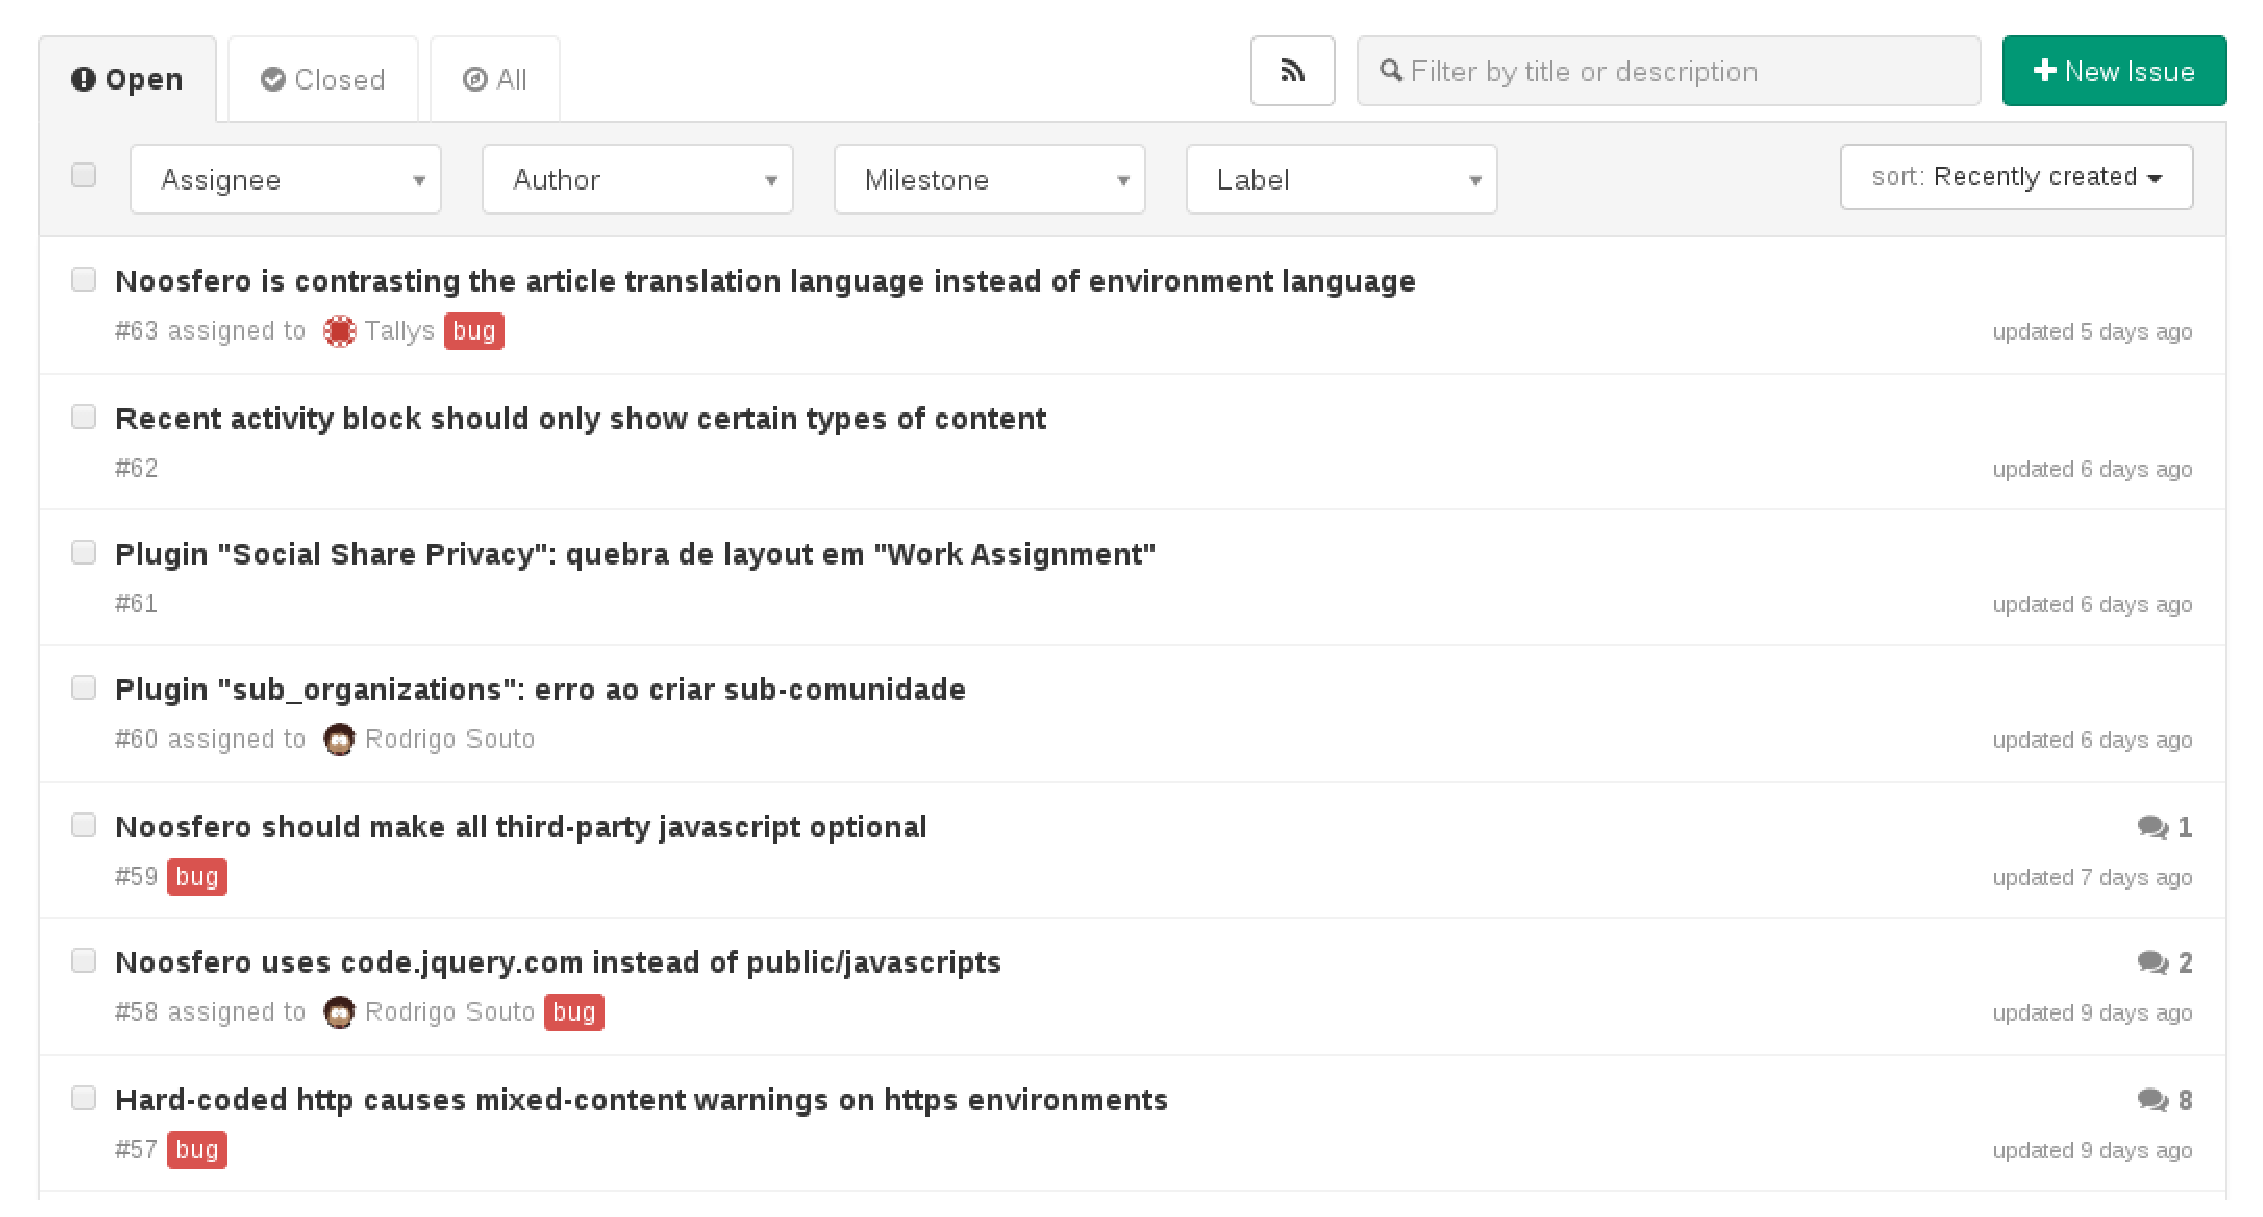
\includegraphics[keepaspectratio=true,scale=0.4]
      {figuras/issueTrackerGitLab.eps}
    \caption{Issue Tracker no GitLab}
    \label{issue-tracker}
\end{figure}

A implementação é realizada pelo desenvolvedor que tem a responsabilidade de manter a qualidade do código produzido bem como todos os testes relacionados à funcionalidade implementada. Uma vez que este primeiro passo esteja concluído o código é submetido a um \textit{merge-request} onde algum dos desenvolvedores do \textit{core} revisa para verificar se está de acordo com os padrões esperados, e aprova ou não, a inclusão do código na \textit{branch} principal do Noosfero.

A comunidade Noosfero adota e recomenda práticas de desenvolvimento como o TDD, \textit{Test Driven Development} ou Desenvolvimento orientado a testes), combinado com o BDD \footnote{\url{https://cukes.info/}} (\textit{Behavior Driven Development}ou Desenvolvimento Guiado por Comportamento, que possibilita o desenvolviemnto de um código tenha uma maior coesão e um menor acoplamento.

Para realizar o controle de versão e gerenciamento do código fonte é utilizado o Git, uma ferramenta livre de versionamento distribuído de código fonte. O repositório oficial do Noosfero encontra-se no software livre Gitlab\footnote{\url{https://gitlab.com/noosfero/noosfero}} com um espelho no Github\footnote{\url{https://github.com/noosfero/noosfero}}. Na página de desenvolvimento da comunidade existe uma série de recomendações sobre como enviar patches para o Noosfero, desde como versionar seu patches, até como realizar a solicitação de inclusão do seu patch, ou \textit{merge-request}, na plataforma.

\subsection{Arquitetura}
\label{arquitetura}
 % Falar porque é importante conhecer a arquitetura do noosfero
Para a evolução de um software de forma adequada é importante o conhecimento da arquitetura do sistema, para não comprometer todo o planejamento realizado na concepção do projeto. Deste modo conhecer e entender a arquitetura de funcionamento do Noosfero, é uma etapa fundamental para o densevolvimento de novas funcionalidades para a plataforma.

 % Conceitos sobre o que é arquitetura
Arquitetura de software são as estruturas do sistema, que abrange os componentes de software, as propriedades externamente visíveis desses componentes e as relações entre elas \cite{pressman2011engenharia}. De acordo com \citeonline{garlan1995introduction} a arquitetura é a estrutura dos componentes de um programa/sistema, suas inter-relações e princípios e diretrizes que regem sua concepção expondo as dimensões através das quais um sistema deve evoluir.

Apesar da existência de variações quanto a definição de arquitetura de software, entende-se que ela está ligada aos módulos do sistema e como eles se relacionam, dessa maneira todos os sistemas possuem alguma tipo de arquitetura.

%Introduzir a figura
Na figura 13, é apresentado a arquitetura básica de funcionamento do Noosfero.
Nessa figura, o solicitante através do seu navegador web (browser) envia uma requisição ao
Noosfero. Essa requisição é tratada pelo Varnish 6 , que repassa ao Apache 7 , que funciona
como um redirecionador para o servidor web do Rails, chamado de Thin 8 . Após isso o
Action Dispacher trata a requisição e envia ela para a controladora responsável.

Na figura \ref{arquitetura-noosfero}, é apresentado uma visão alto nível da arquitetura do Noofero. Basicamente tem-se uma arquitetura cliente-servidor onde o cliente via \textbf{\textit{Browser}} solicita um conteúdo ou uma função para o servidor Noosfero, que aguardam requisições de entrada para processá-las e compartilhar recursos com o cliente.

\begin{figure}[h]
    \centering
    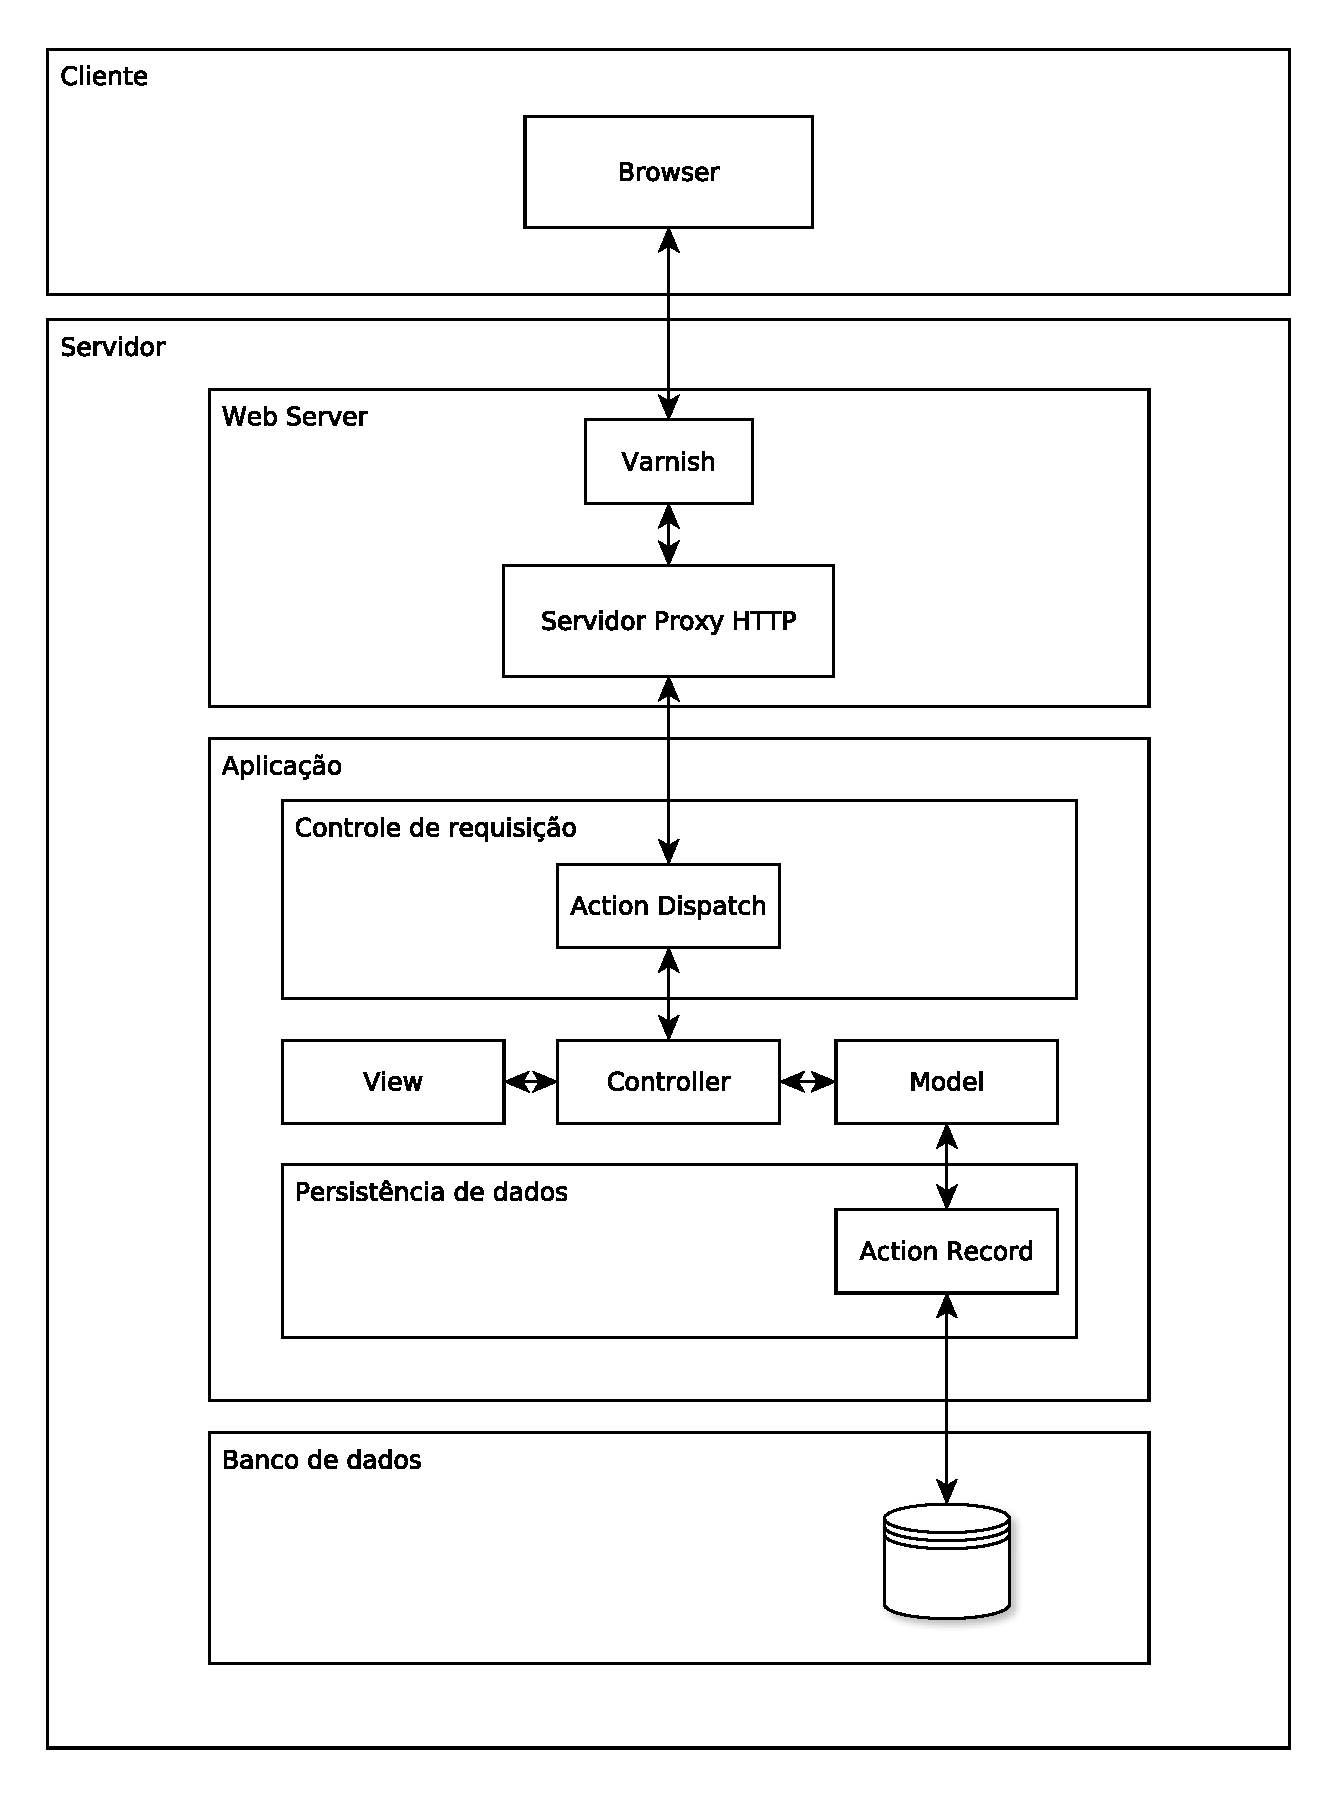
\includegraphics[keepaspectratio=true,scale=0.4]
      {figuras/DiagramaDeArquitetura.eps}
    \caption{Arquitetura do Noosfero}
    \label{arquitetura-noosfero}
\end{figure}

Do lado do servidor temos basicamente três camadas de abstração: \textit{Web-Server}, \textit{aplicação} e \textit{Banco de dados}. Na primeira camada temos dois componentes responsáveis por processar e acelerar todas as requisições de entrada e saída, os componenentes são:
\begin{itemize}
\item Varnish: é um acelerador para sites web dinâmicos com alto volume de conteúdo que utiliza proxy HTTP Reverso. Sua efiência deve-se ao fato dele armazenar o conteúdo HTTP requisitado na memória RAM, fazendo com que o servidor não consulte e processe diversas vezes o mesmo conteúdo solicitado.
\item Servidor Proxy HTTP: pode ser utilizado o Apache ou Nginx \footnote{\url{http://nginx.org}} que ajudam a melhorar o desempenho funcionando como um servidor proxy HTTP reverso que processa as requisições de entrada e saída e as encaminha para a aplicação executá-las.
\end{itemize}

Na camada da aplicação foi considerada uma camada responsável pelo controle de requisições, que é efetuada pelo componente \textbf{\textit{Action Dispatch}}, que lida com o mapeamento de todas as requisições, \textit{cookies} e sessão para suas respectivas \textit{controllers}.

Na aplicação utiliza-se o padrão de arquitetura de software MVC\footnote{Model-view-controller} onde a \textbf{\textit{controller}} controla o fluxo da aplicação. Relacionando as entidades de \textit{model} e de \textit{view} através de chamadas de métodos.A \textbf{\textit{model}} representa as entidades do domínio da aplicação, onde a lógica do sistema são implementadas. A \textbf{\textit{view}} é a interface de comunicação com o usuário, ou seja as páginas HTML apresentadas no navegador.

Ainda na camada da aplicação tem-se o \textbf{\textit{Active Record}} que é um ORM \footnote{object-relational mapping}, ou seja, um mapeador entre objetos e registros de uma tabela, onde cada classe de modelo possui uma tabela correspondente à ela no banco de dados.

E por fim temos a camada de banco de dados que recebe requisições da camada de persistência de dados e por meio de um sistema gerenciador de banco de dados (SGBD) realizam operações na base de dados.

\subsection{Modelo de domínio}

% Falar sobre o modelo de domínio

%Domínio ambiente, domínio e perfis
O Noosfero é uma plataforma que tem suporte a vários ambientes de rede social dentro de uma mesma instalação. Na Figura \ref{domain_main} mostra-se o funcionamento geral do Noosfero com suas quatro principais classes \textbf{\textit{Domain}}, \textbf{\textit{Environment}}, \textbf{\textit{Profile}} e \textbf{\textit{Article}} (Em português: Domínio, Ambiente, Perfil e Artigo respectivamente). Analisando o modelo verifica-se que na implementação é necessário que exista pelo um domínio e partir disso é possível criar várias instâncias de Ambiente na aplicação.

\begin{figure}[h]
    \centering
    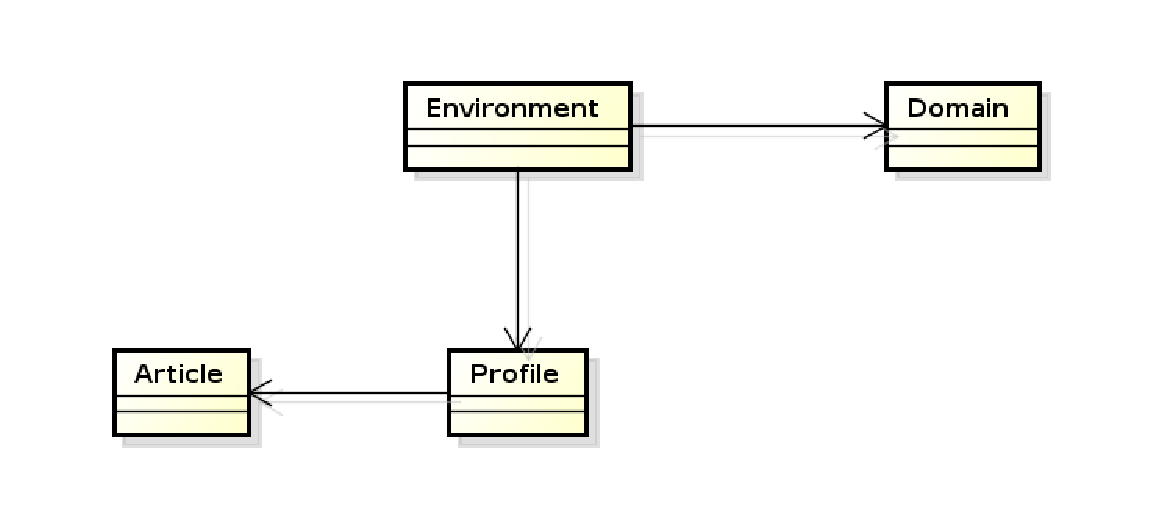
\includegraphics[keepaspectratio=true,scale=0.65]
      {figuras/domain_main.eps}
    \caption{Relações entre entidades de domínio ambiente, domínio e perfis. Extraído de: \cite{bucher2013rede}}
    \label{domain_main}
\end{figure}

A entidade Profile é uma generalização das entidades \textbf{\textit{Person}} (Pessoa) e \textbf{\textit{Organization}} (Organização), como pode ser visto na Figura \ref{domain_profiles}. Nesse mesmo modelo percebe-se que Organization é especializada nas entidades concretas \textbf{\textit{Community}} (Comunidade e Enterprise (Empreendimento). A herança é um mecanismo pelo qual qual uma classe sub-classe pode estender uma super-classe, onde basicamente isola-se métodos ou atributos em comum dentro de uma classe pai (super-classe), enquanto as especialidades são responsabilidade das classes filhas (sub-classe).
%Procurar fonte para herança
Por questões de design do código da aplicação foi criada uma entidade \textbf{\textit{User}}, ou Usuário, que é mantida separada da entidade Pessoa, que é quem implementa a lógica de autenticação da aplicação. Desta forma a lógica de autenticação fica separada da lógica de visualização e personalização do perfil.

\begin{figure}[h]
    \centering
    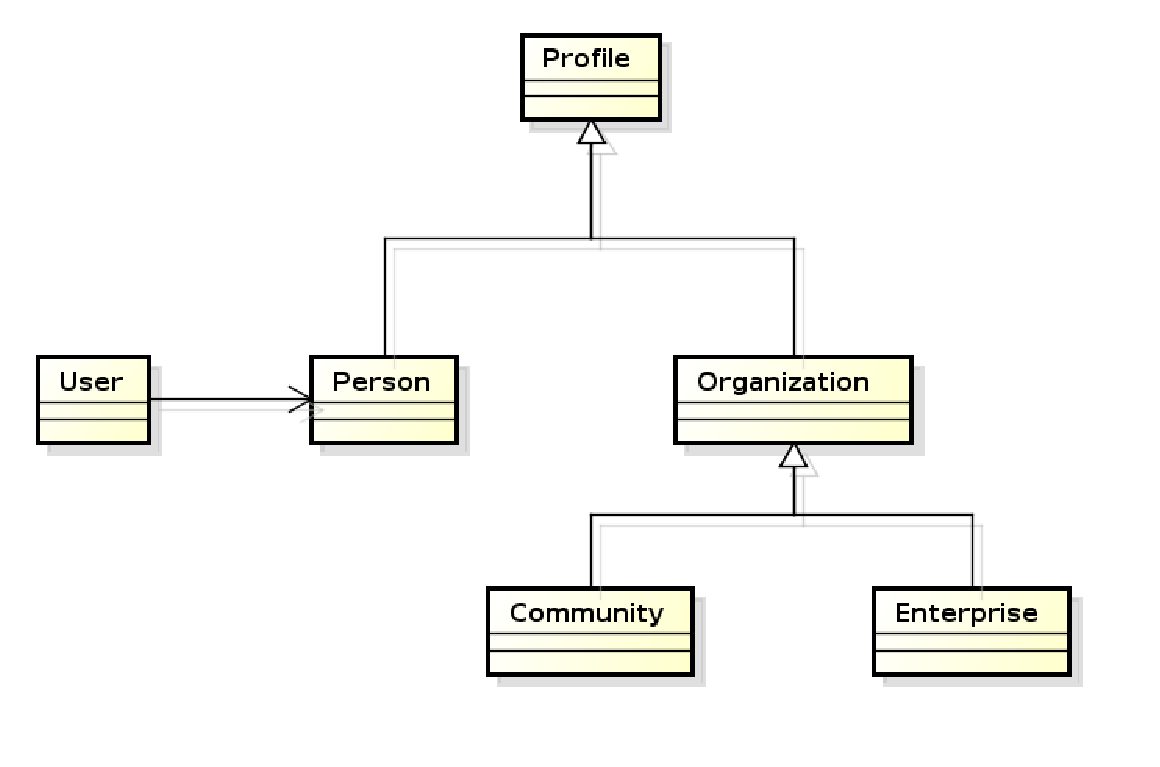
\includegraphics[keepaspectratio=true,scale=0.6]
      {figuras/domain_profiles.eps}
    \caption{Entidades de domínio: tipos de perfis. Extraído de: \cite{bucher2013rede}}
    \label{domain_profiles}
\end{figure}

Por fim, as entidades mostradas na Figura \ref{domain_articles} representam os principais tipos de conteúdos disponíveis no Noosfero, onde a classe \textbf{\textit{Article}}, ou Artigo, é uma especialização de todos os conteúdos disponíveis como: artigos de texto, pastas, blogs, galerias de imagens, fórum, arquivos e feeds de notícias.

\begin{figure}[h]
    \centering
    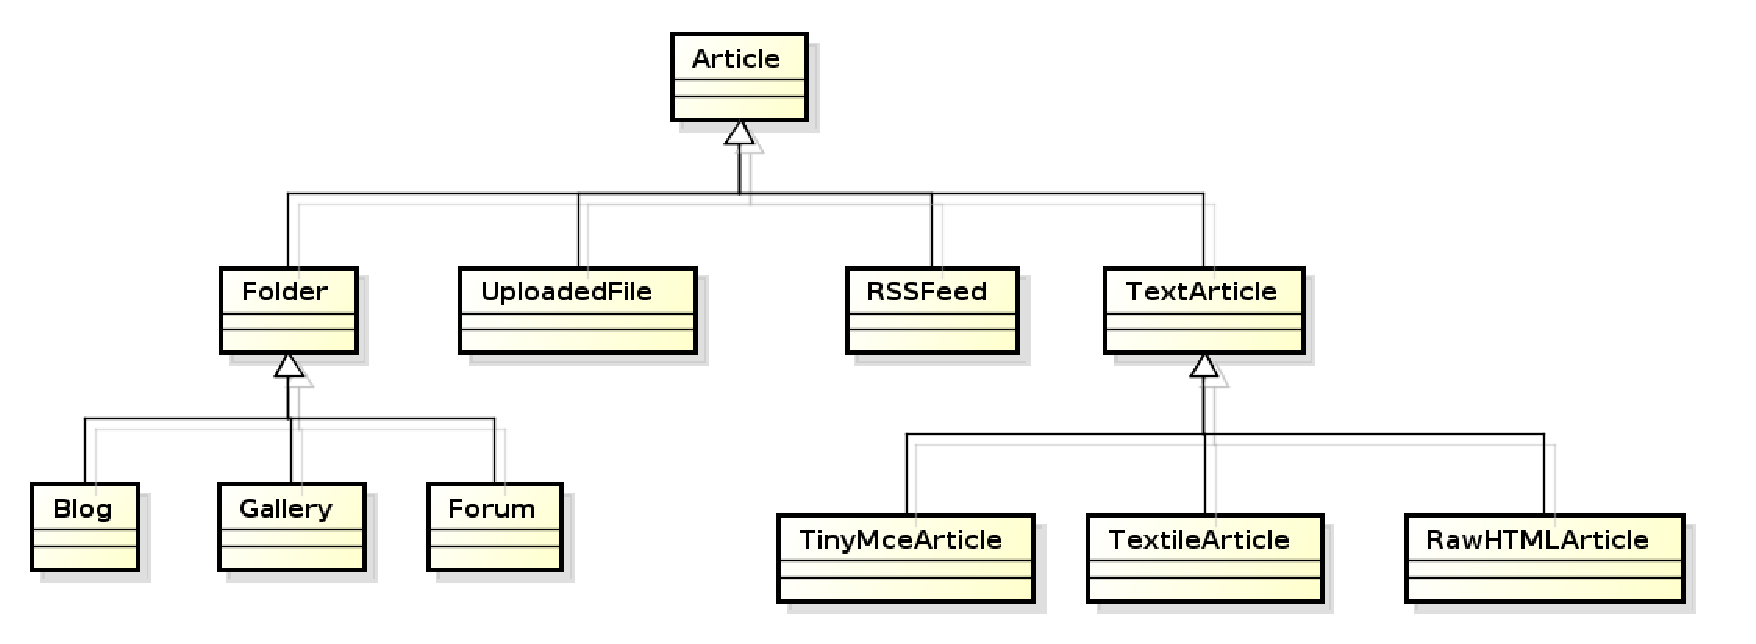
\includegraphics[keepaspectratio=true,scale=0.55]
      {figuras/domain_articles.eps}
    \caption{Entidades de domínio: tipos de artigos. Extraído de: \cite{bucher2013rede}}
    \label{domain_articles}
\end{figure}

% Mesmo com as vantagens do ponto de vista arquitetural e a constante evolução do Noosfero, essa plataforma ainda necessita de algumas melhorias e novas funcionalidades, que foram atendidas, em parte, neste trabalho com a implementação e/ou evolução de plugins, na maioria dos casos de nossas colaborações.

\subsection{Plugins}

Como um software está em constante evolução a arquitetura do Noosfero foi criada para ser altamente expansível fazendo-se o uso de \textit{plugins}. Essa arquitetura permite que em cada ambiente fique a critério do usuário quais os \textit{plugins}, novas funcionalidades, serão habilitadas o que torna o sistema flexível e modular.

\begin{figure}[h]
    \centering
    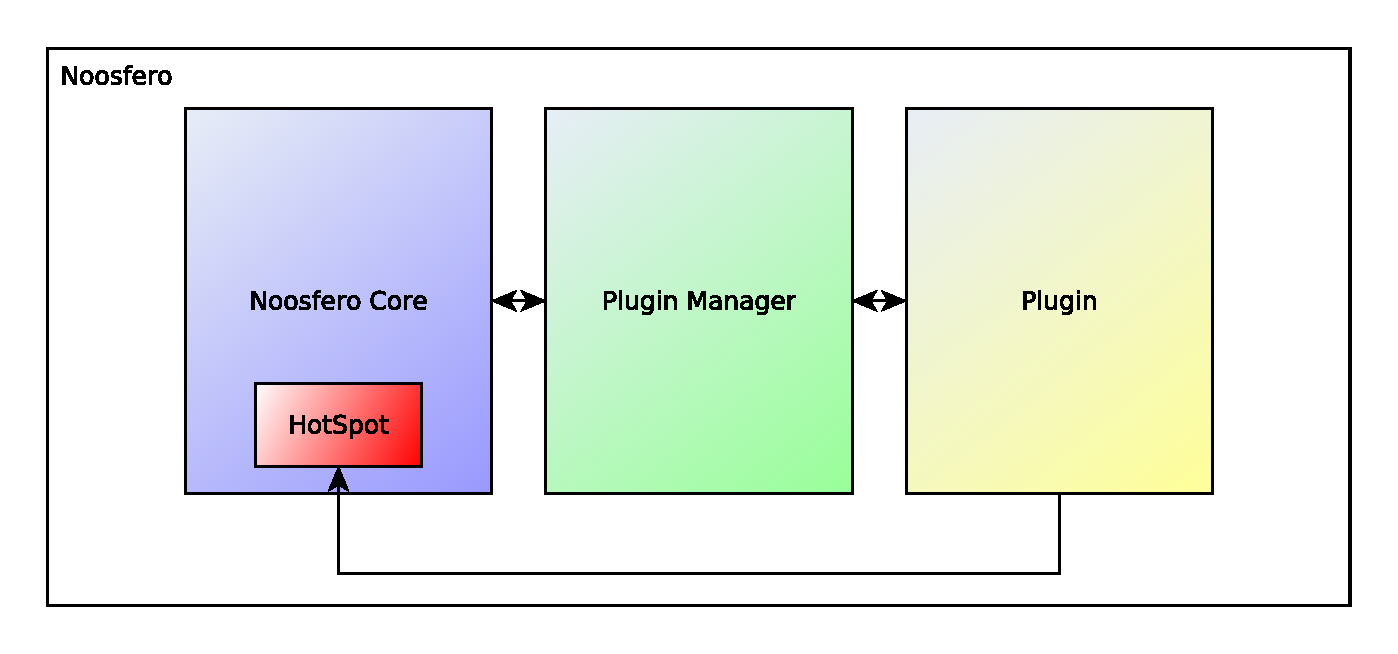
\includegraphics[keepaspectratio=true,scale=0.4]
      {figuras/estruturaDePlugins.eps}
    \caption{Estrutura de Plugins}
    \label{estrutura-plugins}
\end{figure}

A figura \ref{estrutura-plugins} é uma abstração alto nível do funcionamento interno dos plugins no Noosfero. No \textit{core} do Noosfero temos os \textit{hotspots}, que são pontos de flexibilidade o qual permitem associar diferentes comportamentos na execução do sistema, permitindo a inserção de trechos de código e ou alteração de um determinado método sem comprometer as funcionalidades básicas do sistema.

Os \textit{hotspots} são gerenciados por uma camada de abstração denominada \textit{Plugin Manager}, ou Gerenciador de \textit{Plugins}, que são chamadas pelo \textit{core} através de um metódo principal conhecido como \textit{dispatch}. Basicamente o ciclo de execução pode ser descrito da seginte maneira, durante a execução de alguma funcionalidade o método \textit{dispatch} é invocado por alguma funcionalildade do core, deste modo o gerenciador de plugins verifica todos os \textit{Plugins} que fazem uso daquele \textit{hotspot} e encaminha para cada um deles a execução de suas ações de acordo com sua implementação.

Essa arquitetura extensível adotada pelo Noosfero auxilia no controle da qualidade de código das novas funcionalidades. A camada de \textit{Plugins} para o Noosfero é uma que fica o código do seu núcleo, localiza-se em uma pasta denominada \textit{plugins} em que desenvolvedor cria novas funcionalidades sem modificar o \textit{core} do Noosfero.

Como mencionado na seção \ref{proc-desenvol-comunidade} o Noosfero faz uso de testes para manter a integridade de seu cógido, dessa maneira também é necessário que os \textit{plugins} contenham seus respectivos testes para evitar a inserção de \textit{bugs} e mudanças inesperadas no comportamento do sistema.

\subsection{Comunidade UnB}
\label{comunidade-unb}

O Comunidade.UnB é uma rede colaboração livre desenvolvida para que alunos, professores e servidores técnico-administrativos tenham um ambiente virtual de criação e compartilhamento de conhecimento colaborativo. É um ambiente virtual para o compartilhamento de ideias, produção de conteúdo colaborativo de modo que possam publicá-los para que possa ser de utilidade para outras pessoas ou parcelas da sociedade, uma vez que acredita-se que ete é um dos papéis de uma Universidade \cite{bucher2013rede}.

Inspirada na rede social de colaboração Stoa \footnote{Disponível em: \url{https://social.stoa.usp.br/}}, da Universidade de São Paulo (USP), a Comunidade.UnB foi criada em 2013 a partir de um trabalho de conclusão de curso de Daniel Costa Bucher e até então está disponibilizada em ambiente de testes. O Comunidade.Unb permite ao usuário a criação de seu espaço pessoal e a liberdade de publicar suas ideias, ou o conteúdo que desejar, por exemplo, na forma de blogs pessoais, blogs de disciplinas, pesquisas em andamento, dentre outras, além de compartilhar esse conteúdo para ser acessível para outros usuários dentro e fora da rede.

O Noosfero, descrito na seção \ref{noosfero}, foi a plataforma utilizada para o desenvolvimento do Comunidade.UnB, por dispor de um grande potencial devido as suas funcionalidades avançadas, que permitem a criação e o compartilhamento de conteúdo de forma satisfatória. Além de dispor de uma comunidade ativa e de posição geográfica favorável em relação ao seu núcle de desenvolvimento que se encontra no Brasil, facilitando a comunicação com os seus principais desenvolvedores.

Apesar da Comunidade.UnB estar disponibilizada como um ambiente de testes e não possuir uma vasta divulgação pela Univerdade de Brasília, no seu primeiro ano de criação contava com 153 usuários e 14 comunidades, analisando os novos números contabilizados até o presente momento, 370 usuários e 30 comunidades, nota-se que houve uma duplicação dos números o que indica que o seu uso, mesmo que discretamente, está em crescimento.

Alguns professores adotaram o Comunidade.UnB como um ambiente de apoio ao Moodle, AVA oficial adotado pela UnB, na figura \ref{comunidade-mes} é apresentado um exemplo de seu uso na disciplina de Manutenção e Evolução de Software (MES) ministrada pelo professor Paulo Roberto Miranda Meirelles.

\begin{figure}[!htb]
    \centering
    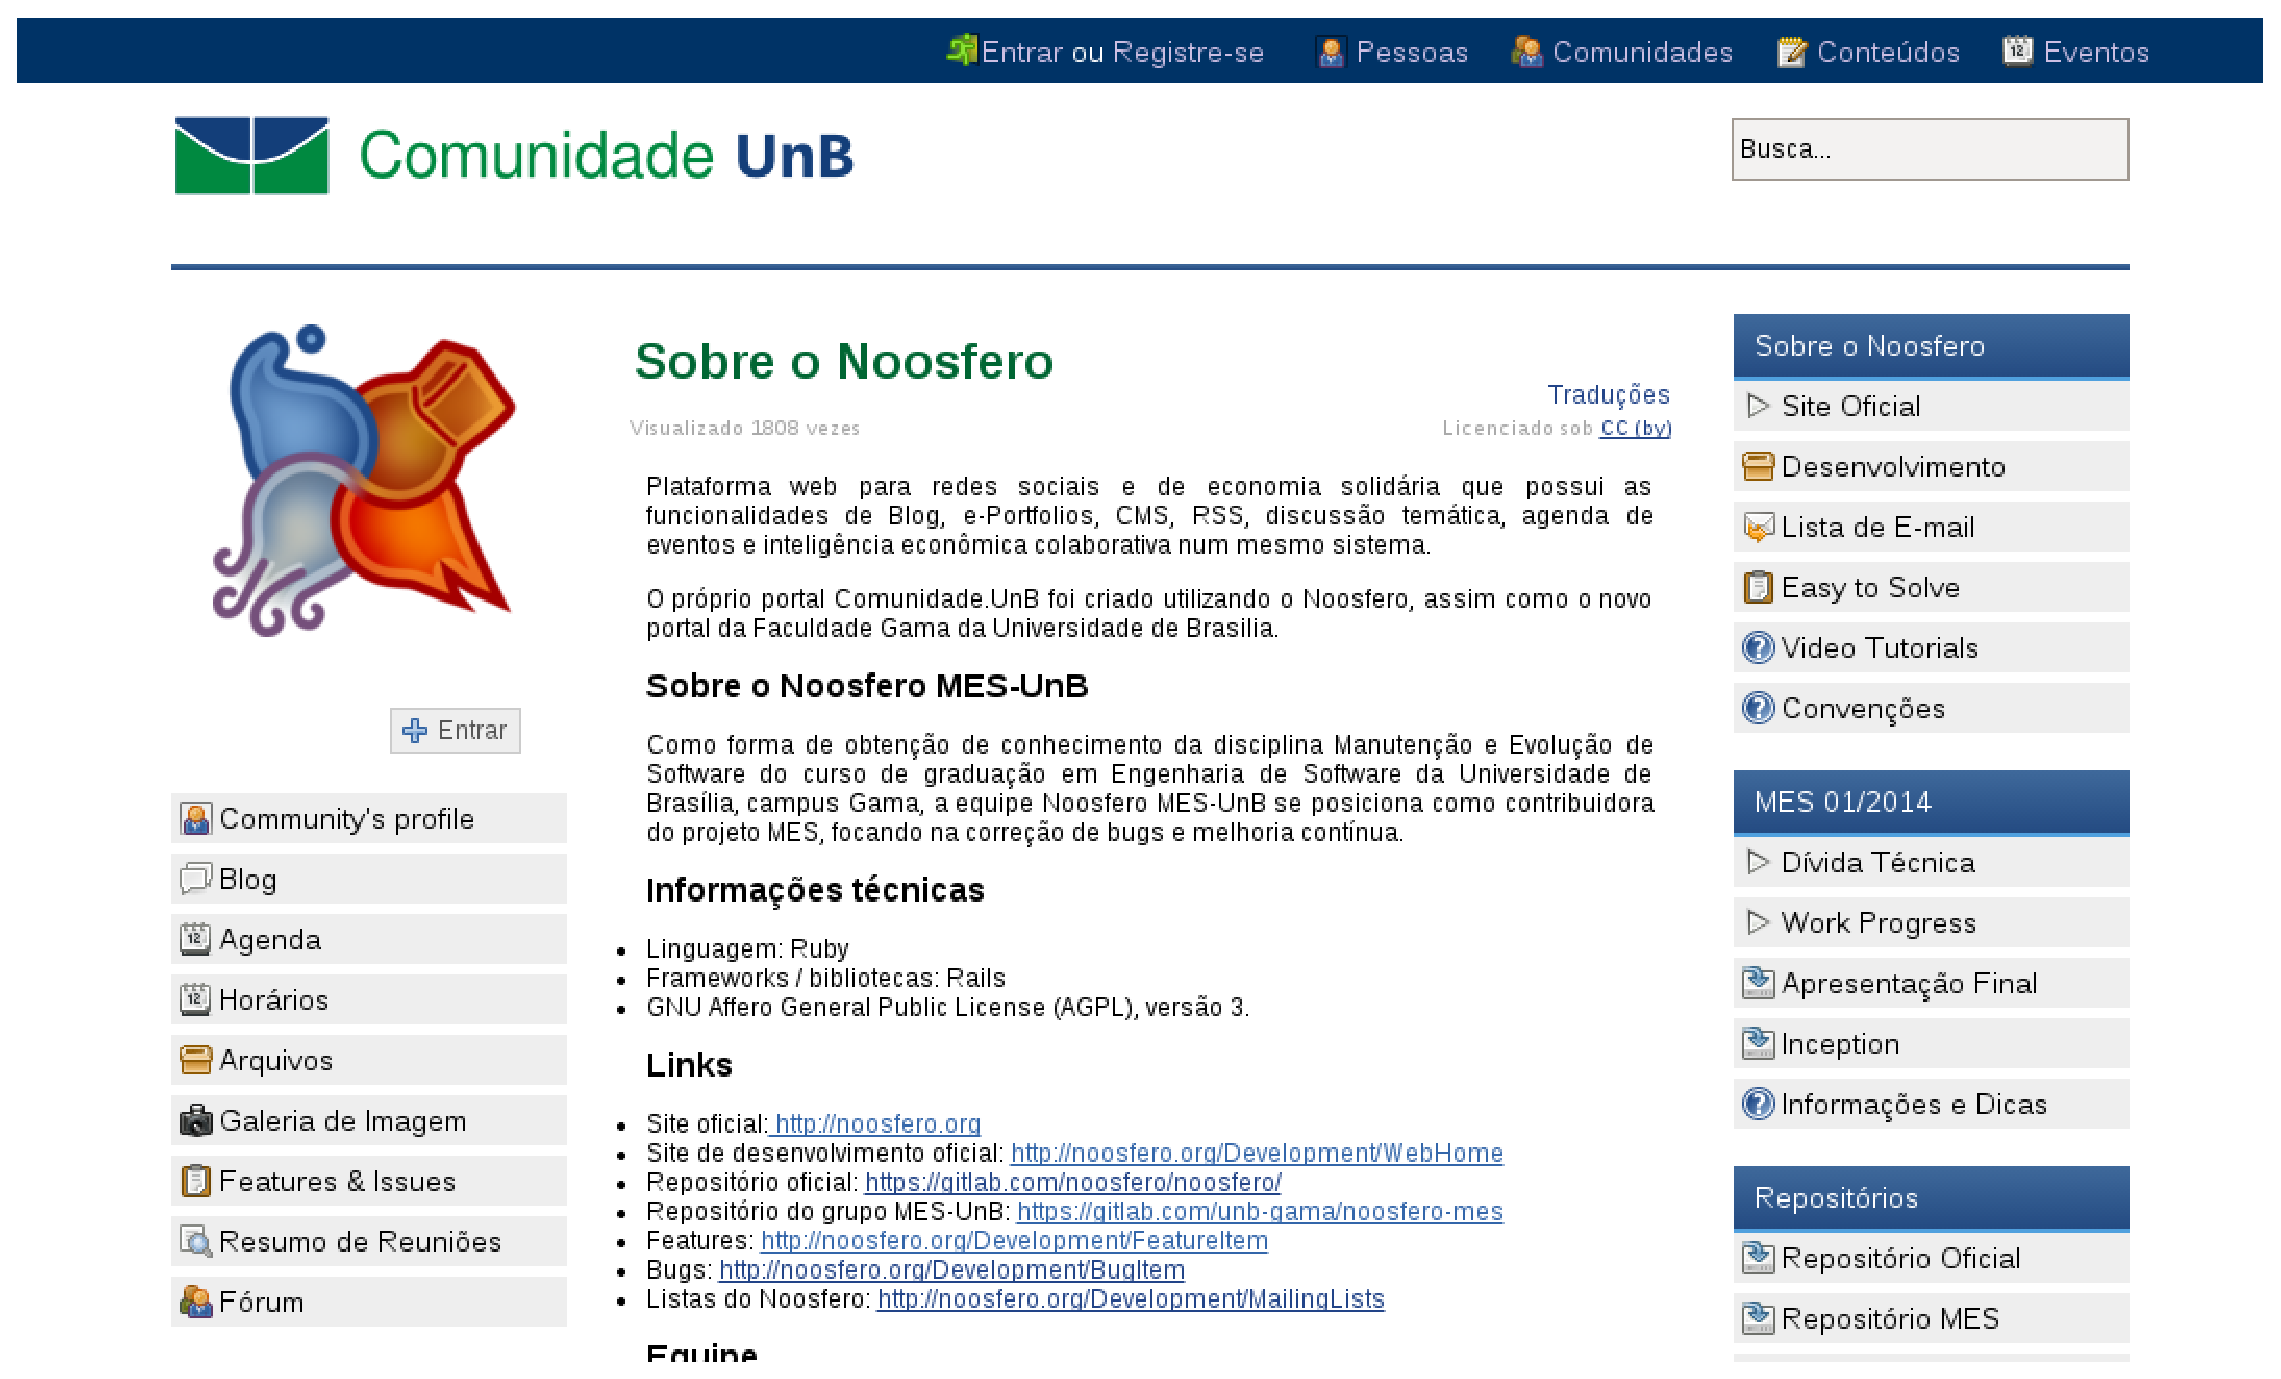
\includegraphics[keepaspectratio=true,scale=0.4]
      {figuras/comunidade-mes.eps}
    \caption{Exemplo do uso do Comunidade.UnB na disciplina de MES.}
    \label{comunidade-mes}
\end{figure}

Este é um exemplo de comunidade criada dentro do Comunidade.UnB, que possui características que se assemelham ao ambiente Moodle, como evidenciado na seção \ref{comparacao-ava}, carecendo de alguns funcionalidades importantes mas com a vantagem da possibilidade de acesso do público ao conteúdo, e a continuidade do conteúdo desenvolvido por outras pessoas que eventualmente se juntem ao longo do tempo. E vale lembrar que em uma publicação de conteúddo os níveis de privacidade podem ser alterados basicamente entre públicos e privados.

Sabendo das limitações apresentadas pela plataforma e a proposta de uso da Comunidade.UnB por professores para a criação de disciplinas, é um fator que estimula o desenvolvimento de funcionalidades que levam à plataforma Noosfero de assemelhar-se a um ambiente virtual de aprendizagem. Desta maneira na seção \ref{desen-noosferAVA} busca-se a proposta de estudo desse trabalho no desenvolvimento de funcionalidade para minimizar as diferenças do Noosfero com os ambientes virtuais de aprendizegem.
%
\section{Desenvolvimento do NoosferAVA}
\label{desen-noosferAVA}

Nesse capítulo apresentaremos as funcionalidades desenvolvidas para contribuir
para a adequação do Noosfero como uma rede de colaboração para universidades, os re-
quisitos não-funcionais levantados para que esta possa suprir as necessidades de segurança
e confiabilidade e o processo de colaboração com o Noosfero. O capítulo 6, na seção de
trabalhos futuros, apresenta outras funcionalidades que foram levantadas por nós mas não
foram desenvolvidas ao longo deste trabalho.

- requisitos
-- funcionalidades adaptadas/melhoras
-- novas funcionalidades

-Atualizar pro rails 3

-Utilização do LDAP
	-realizar melhorias
		-cadastro de matricula dos usuários já existentes
		-

-Evolução do workassigment
	-permitir atribuição de notas para a atividade
	-**timer (plugin de tolerância e tempo)

-*Calendário de atividades
	-Arquivos do work assigment

-Definir template de disciplina

-Sistema de notas